%\documentclass[aspectratio=169]{beamer}
\documentclass{beamer}

\usetheme{mpcshpc}

\usepackage{lmodern}
\usepackage{listings}
\usepackage{hyperref}
\usepackage[scale=2]{ccicons}
\usepackage{minted}
\usepackage{multirow}
\usepackage{graphicx}
\usepackage{caption}
\usepackage{amsmath}
\usepackage{biblatex}
\usepackage{makecell}
\graphicspath{{./img/}}

\title{Lecture 3: Intro to GPUs and CUDA}
\subtitle{MPCS 51087: High-Performance Computing}
\date{Winter 2021}
\author{Ron Rahaman}
\institute{The University of Chicago, Dept of Computer Science}

\setwatermark{
\includegraphics[height=7cm]{img/snail-rocket.png}}
\setminted{fontsize=\footnotesize}

\AtBeginSection[]
{
\begin{frame}
    \frametitle{Table of Contents}
    \tableofcontents[currentsection]
\end{frame}
}


\AtBeginSubsection[]
{
\begin{frame}
    \frametitle{Table of Contents}
    \tableofcontents[currentsubsection]
\end{frame}
}


\begin{document}

    \maketitle

    \begin{frame}
        \frametitle{Table of Contents}
        \tableofcontents[]
    \end{frame}

    \section{Concepts}

    \begin{frame}{GPU Processors}
            CPUs and GPUs each have independent processors that run in parallel:
            \begin{itemize}
                \item CPU: Cores
                \item GPU: Streaming multiprocessors (SM) containing streaming processors (SP)
            \end{itemize}
        \begin{figure}
            \centering
            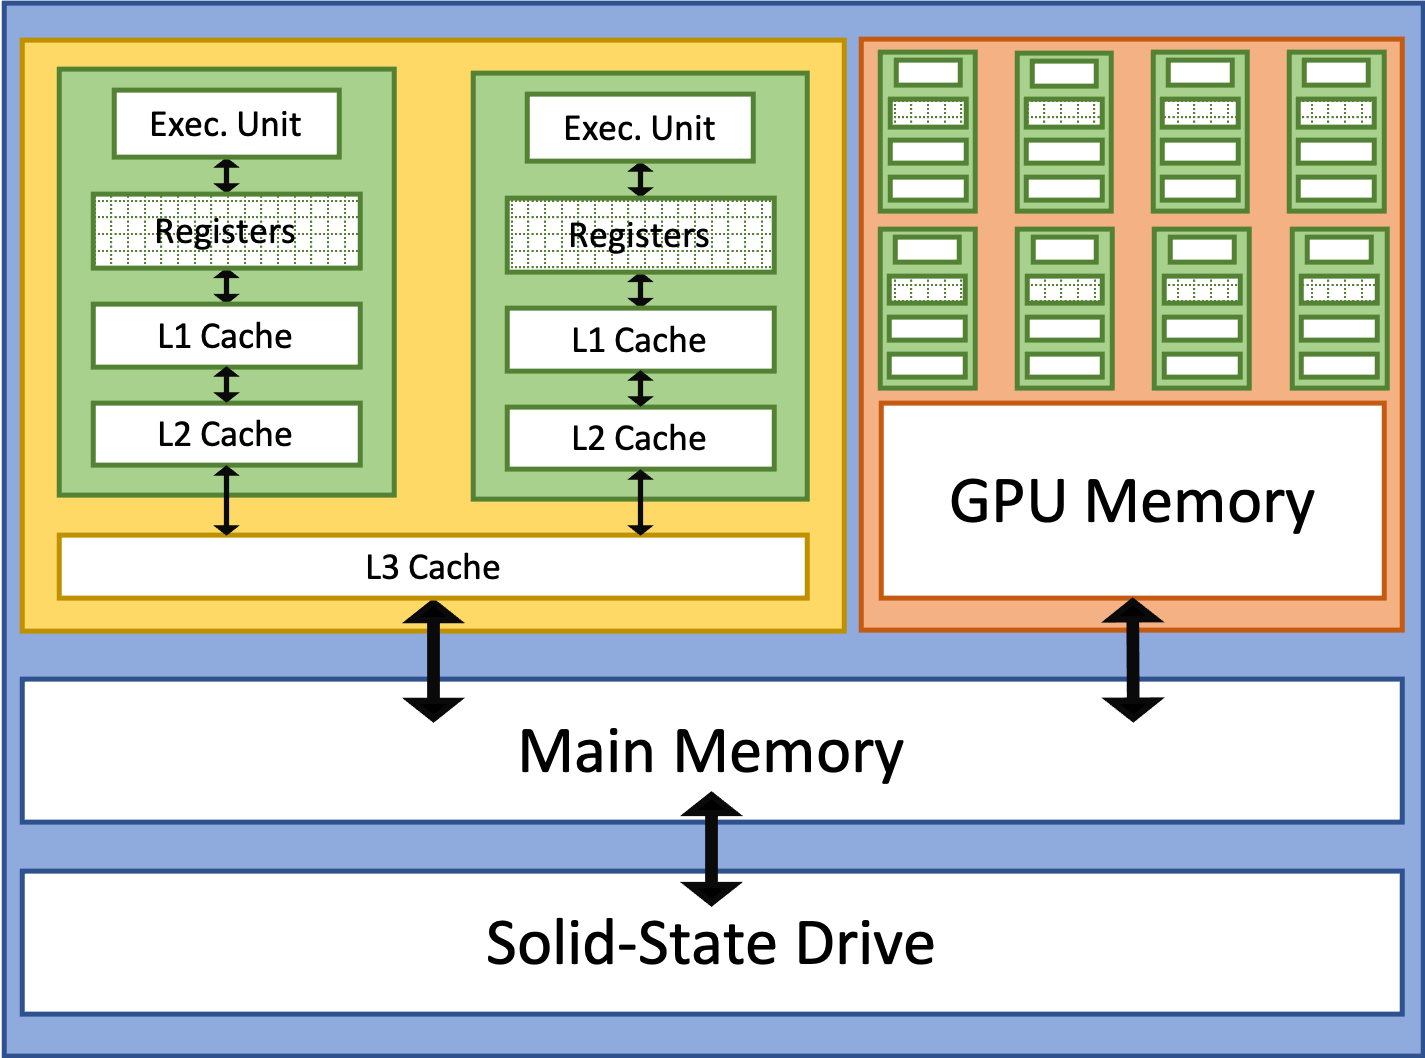
\includegraphics[width=0.6\textwidth]{img/01/mem_hier_node_gpu.png}
        \end{figure}
    \end{frame}

    \begin{frame}{Basic Characteristics of SMs and SPs}
        Some important differences of GPU processors
        \begin{itemize}
            \item Less control logic
            \item Lower clock rates (1.3 GHz on V100)
            \item \textbf{Very fast context switching between threads}
        \end{itemize}
        The fast context-switching hides memory stalls and maximizes throughput
    \end{frame}

    \begin{frame}{GPU Processors}
        \begin{itemize}
            \item CPUs and GPUs both have a cache hierarchy
            \item GPU cache reads from GPU memory (dynamic access memory, DRAM), rather than normal RAM
            \begin{itemize}
                \item DRAM is smaller (16 GB on V100)
                \item DRAM has much higher bandwidth (900 GB/s on V100)
            \end{itemize}
        \end{itemize}
        \begin{figure}
            \centering
            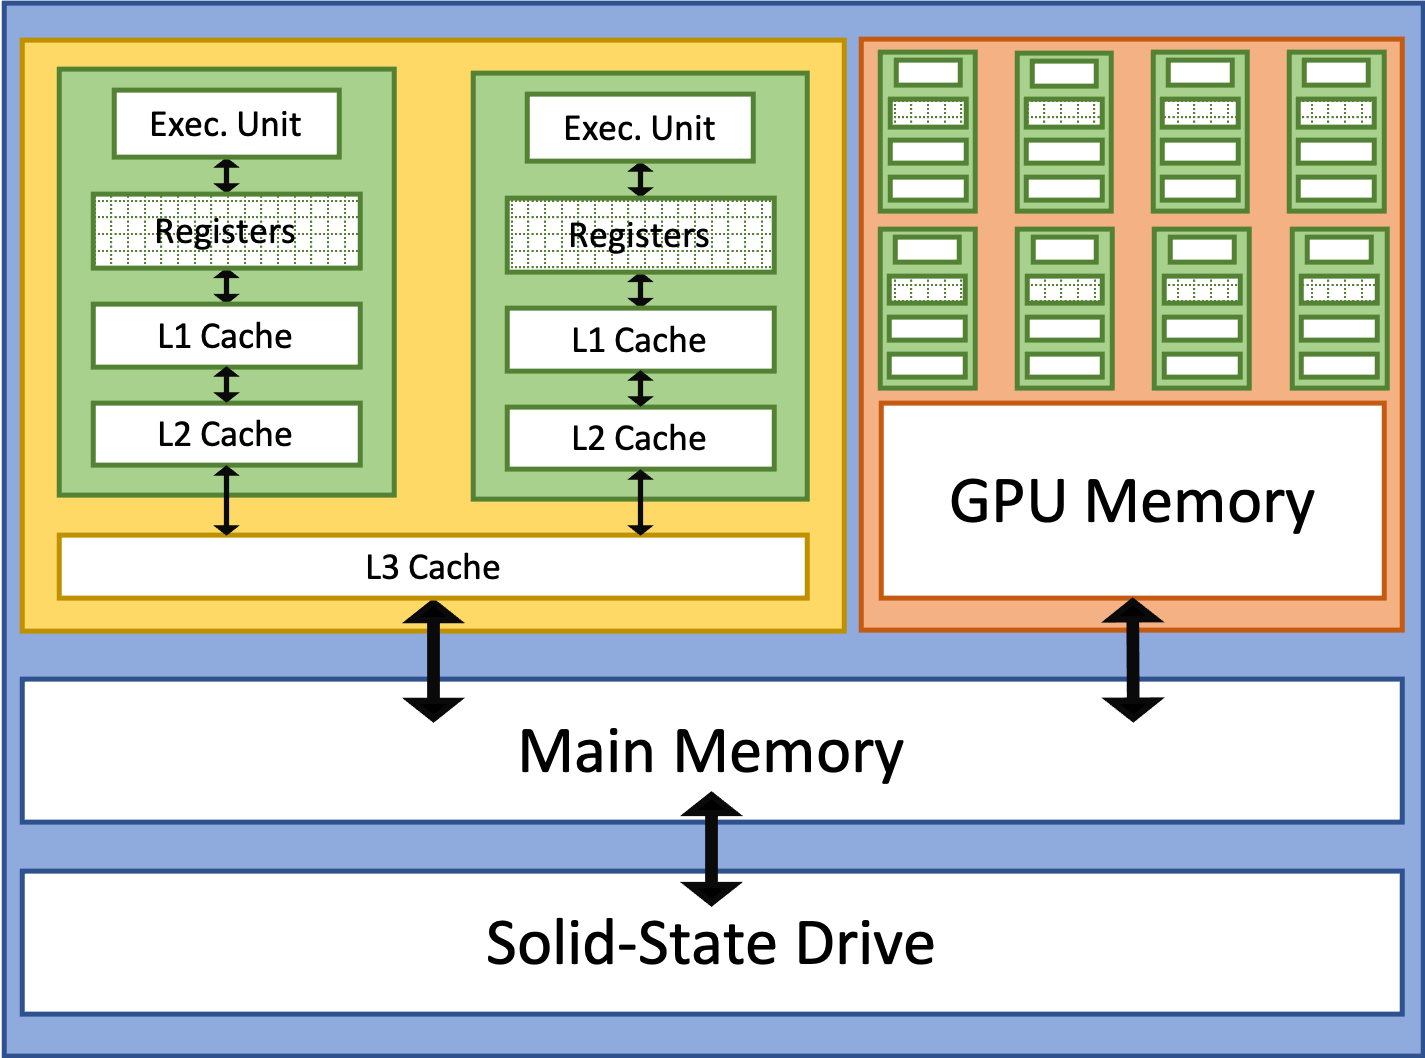
\includegraphics[width=0.6\textwidth]{img/01/mem_hier_node_gpu.png}
        \end{figure}
    \end{frame}

    \begin{frame}{All the Symmetric Multiprocessors (SMs)}
        This is the V100 (Volta), a last-gen GPU that's still high-end
        \begin{itemize}
            \item 80 SMs (green)
            \item L2 shared among all SMs
        \end{itemize}

        \begin{figure}
            \centering
            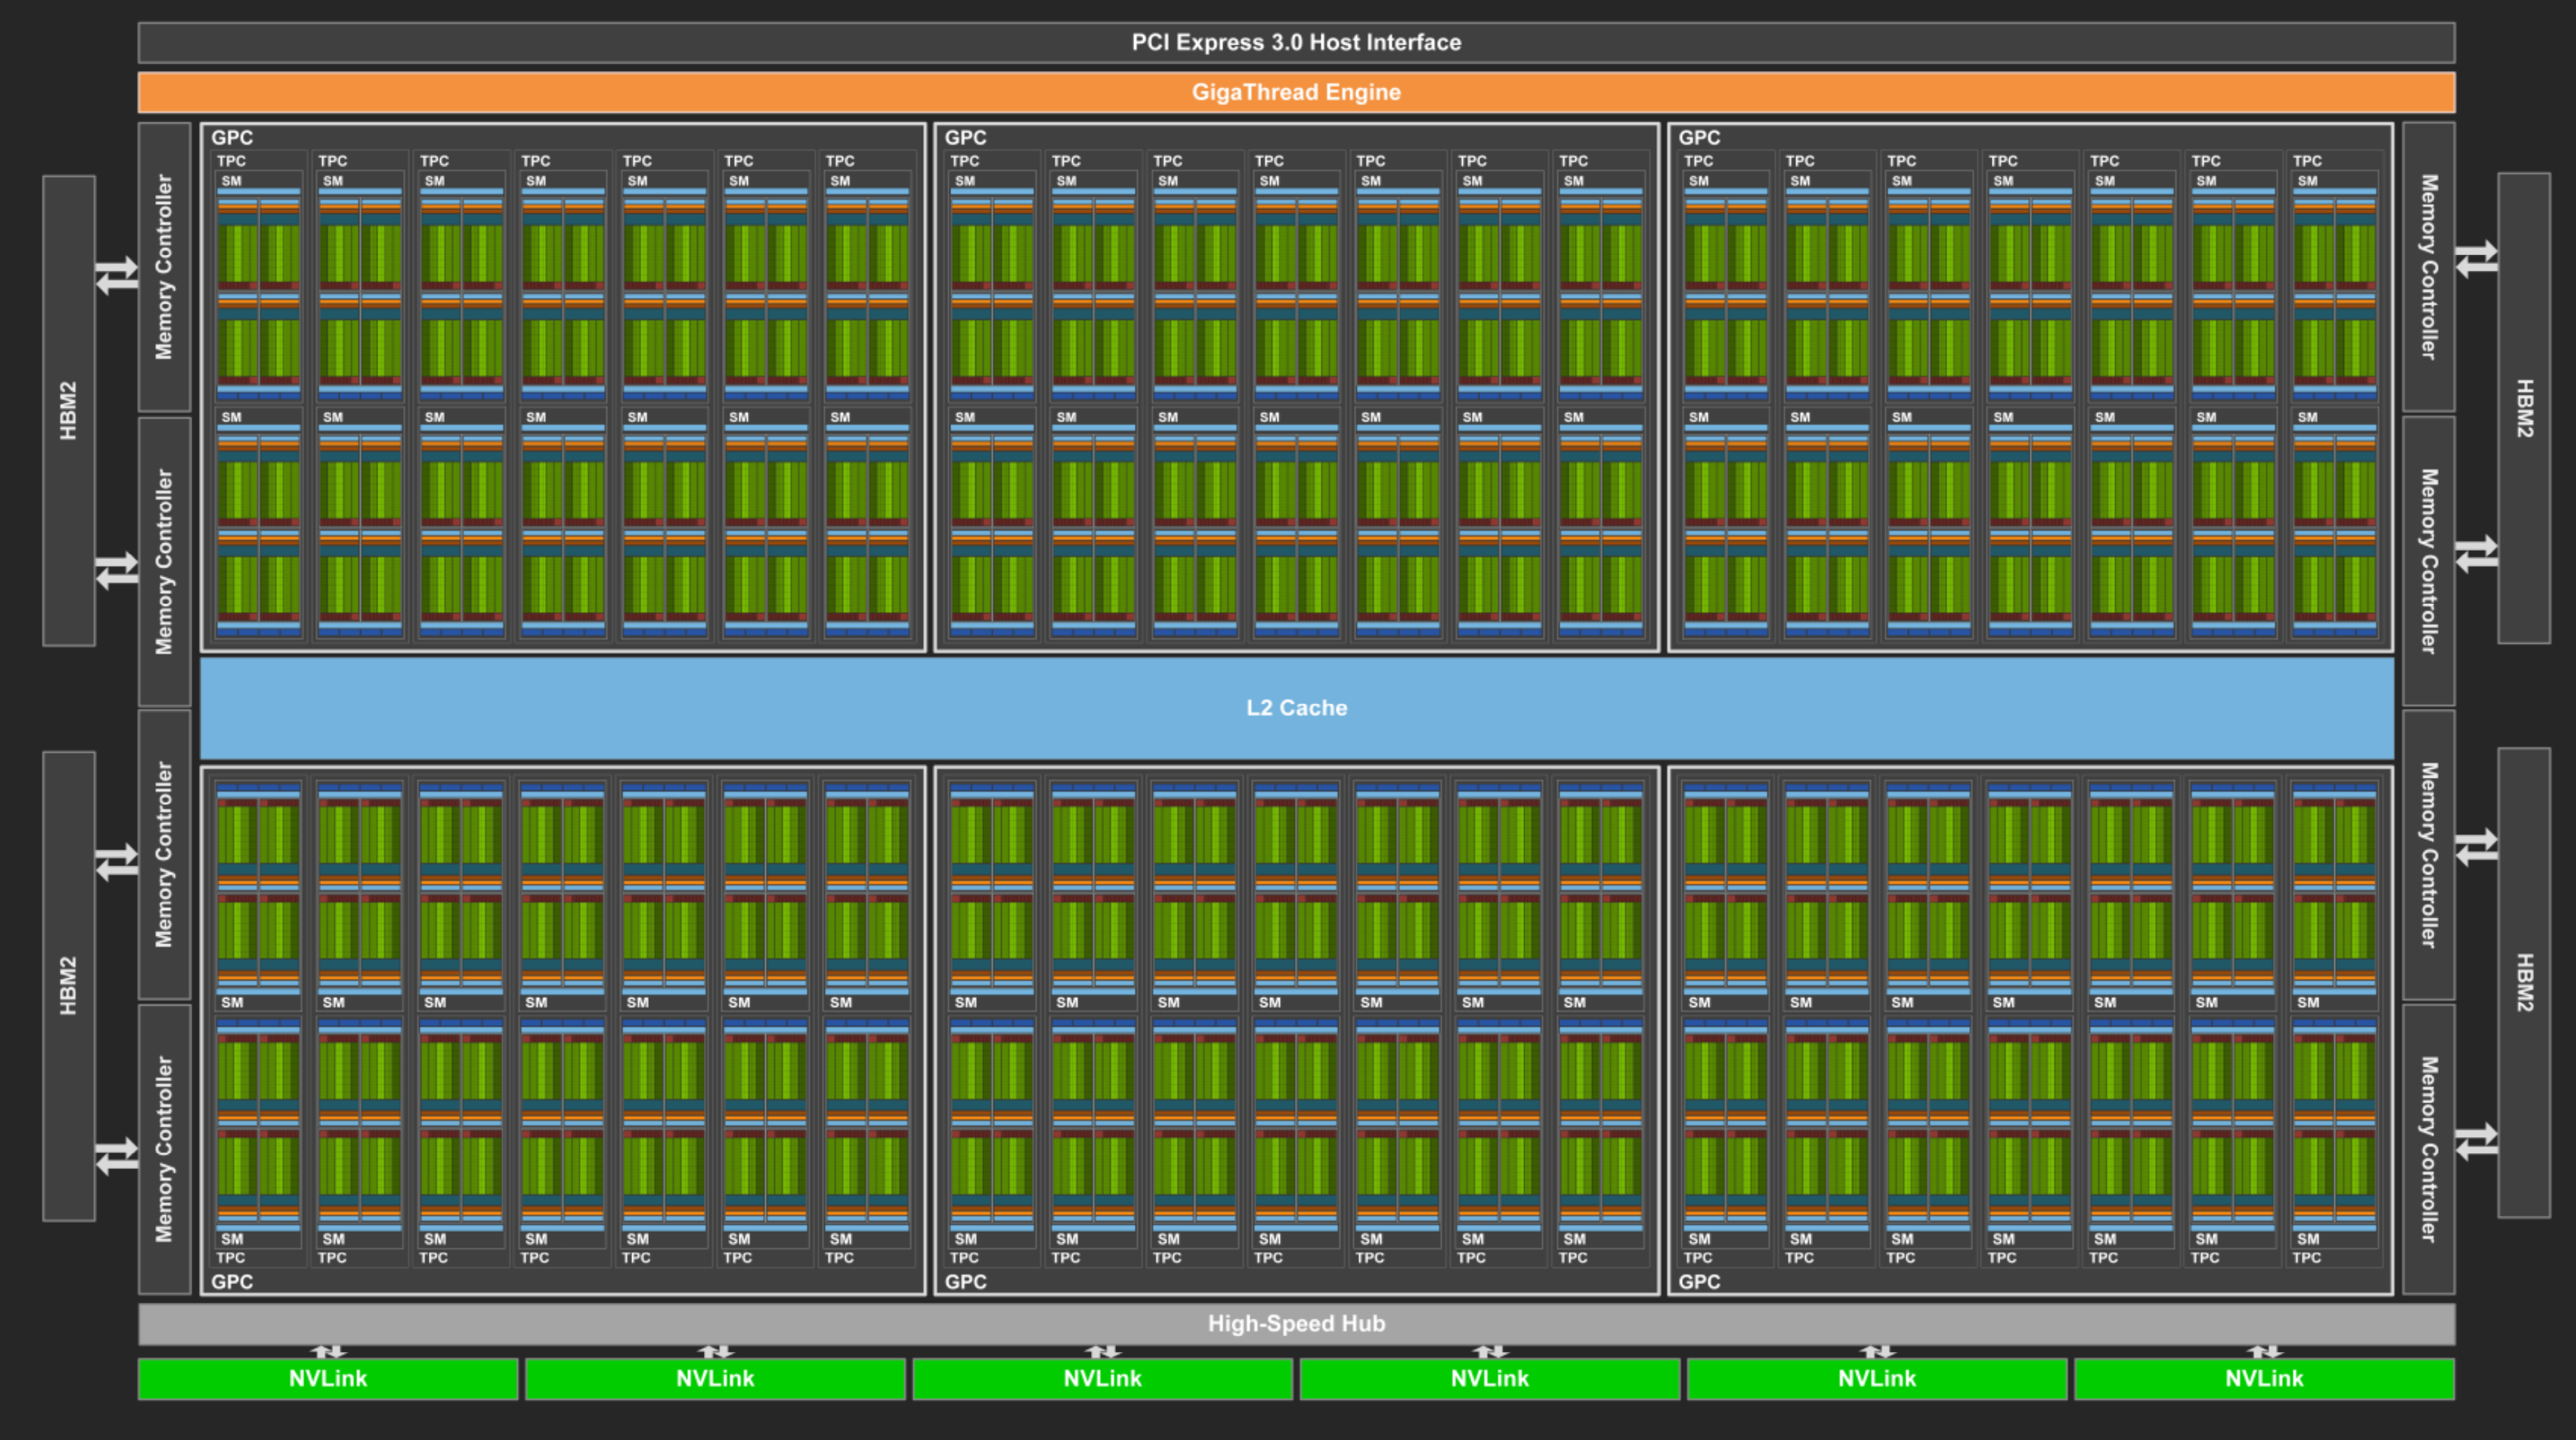
\includegraphics[width=\textwidth]{img/03/volta-smps.png}
        \end{figure}
    \end{frame}

    \begin{frame}{One Symmetric Multiprocessor}
        \begin{columns}
            \column{0.5\textwidth}
            \begin{itemize}
                \item A single SM contains several SPs:
                \begin{itemize}
                    \item 64 integer units
                    \item 64 single-precision units
                    \item 32 double-precision units
                    \item 8 tensor cores
                \end{itemize}
                \item \textbf{A single instruction can be applied to multiple SPs at once}
                \item \textbf{This is how SIMD is implemented on a GPU}
            \end{itemize}
            \column{0.5\textwidth}
            \begin{figure}
                \centering
                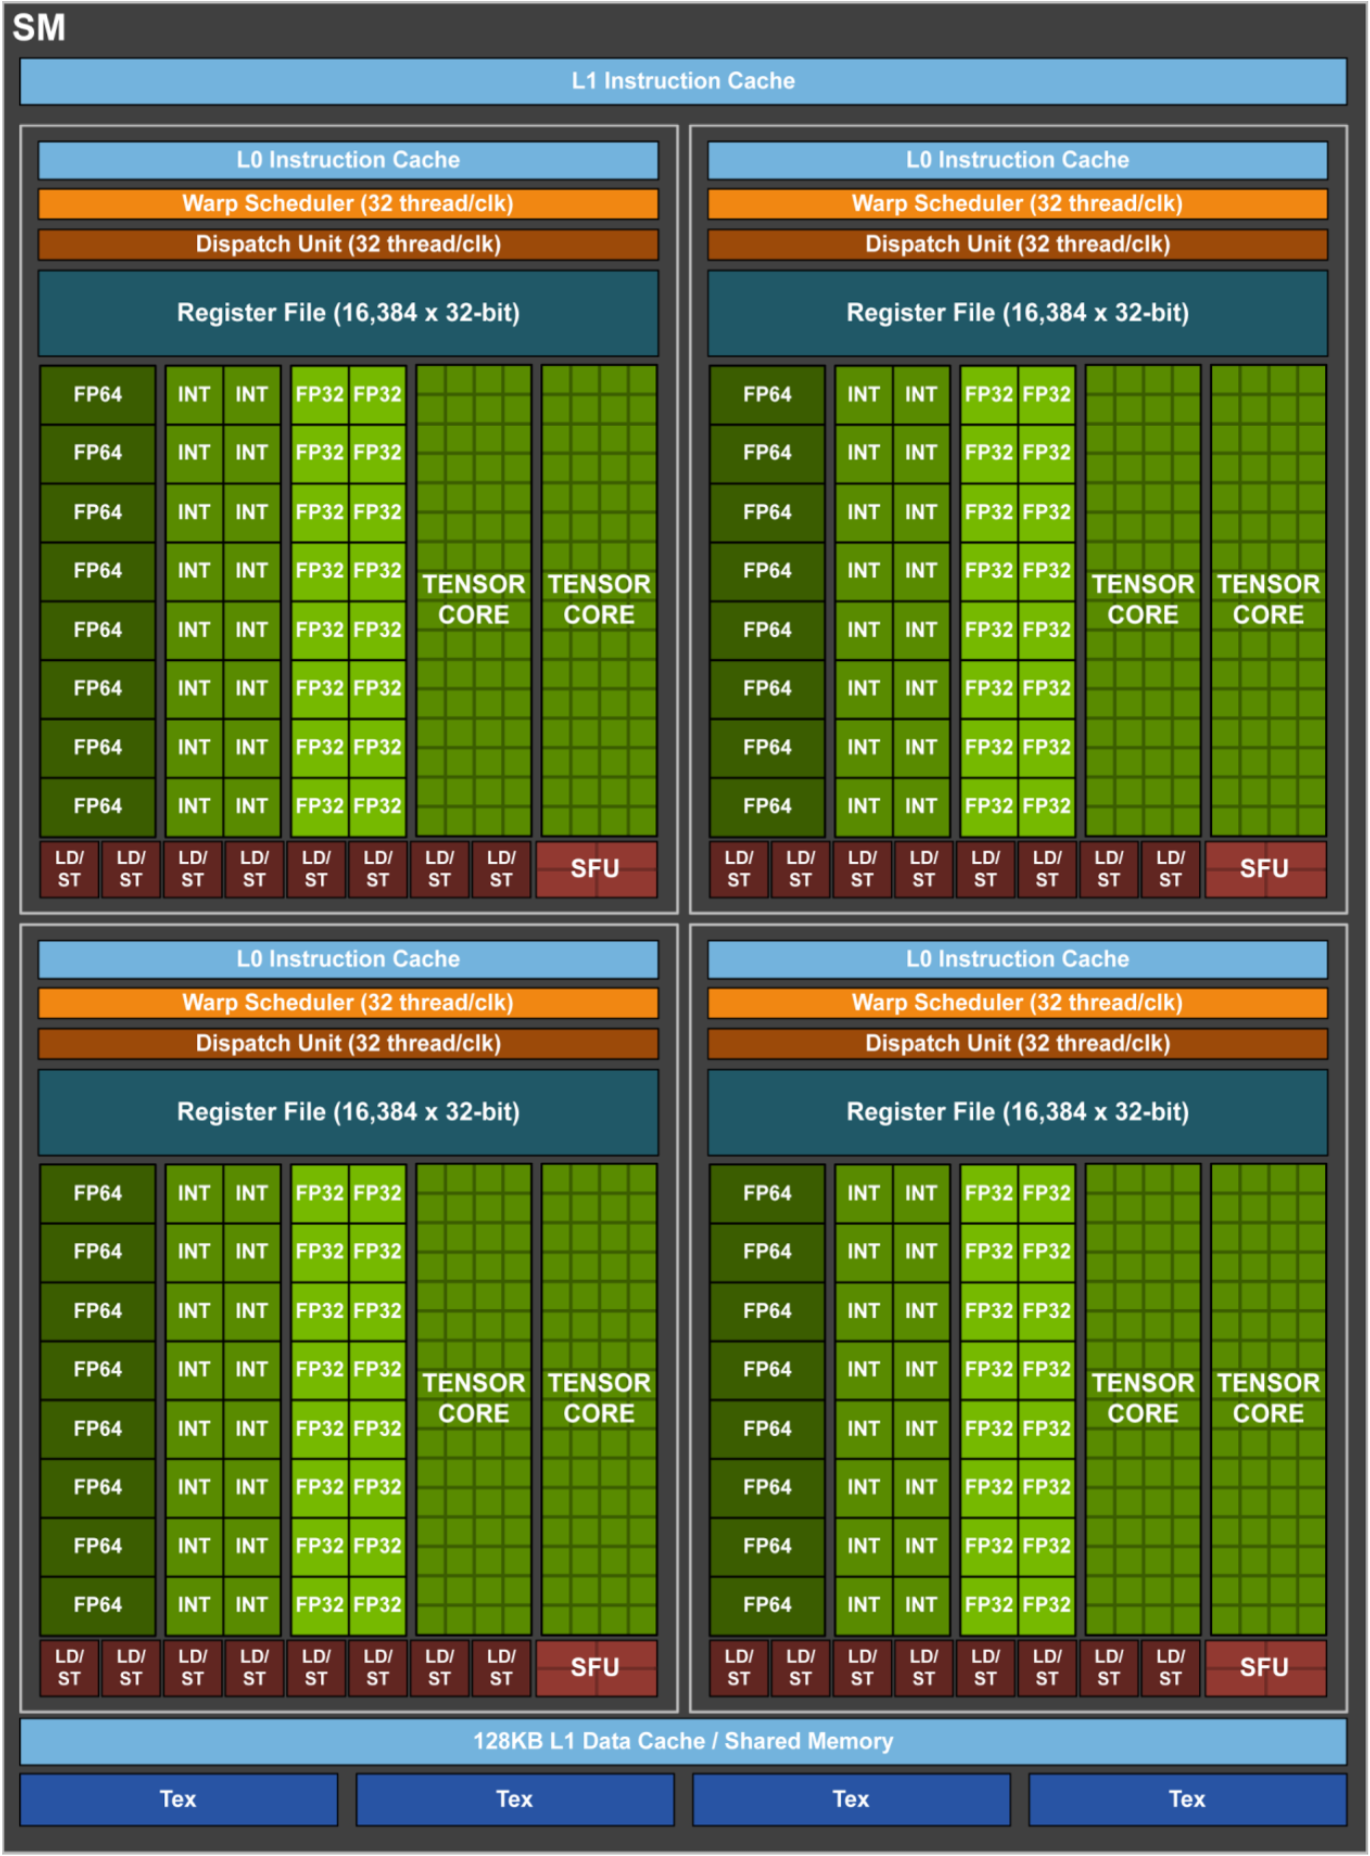
\includegraphics[width=\textwidth]{img/03/volta-sps.png}
            \end{figure}
        \end{columns}
    \end{frame}

    \begin{frame}{Abstraction/Hardware Mapping}
        \begin{columns}
            \column{0.4\textwidth}
            \begin{itemize}
                \item Programming abstractions in CUDA:
                \begin{itemize}
                    \item \textbf{Thread (yellow)}: Runs a single operation on one SP (greem)
                    \item \textbf{Warp (yellow)}: A group of threads that can be executed in SIMD (red)
                    \item \textbf{Block (blue)}: A group of threads and warps that runs on one SM (grey)
                \end{itemize}
                \item These allow multiple levels of parallelism
            \end{itemize}
            \column{0.6\textwidth}
            \begin{figure}
                \centering
                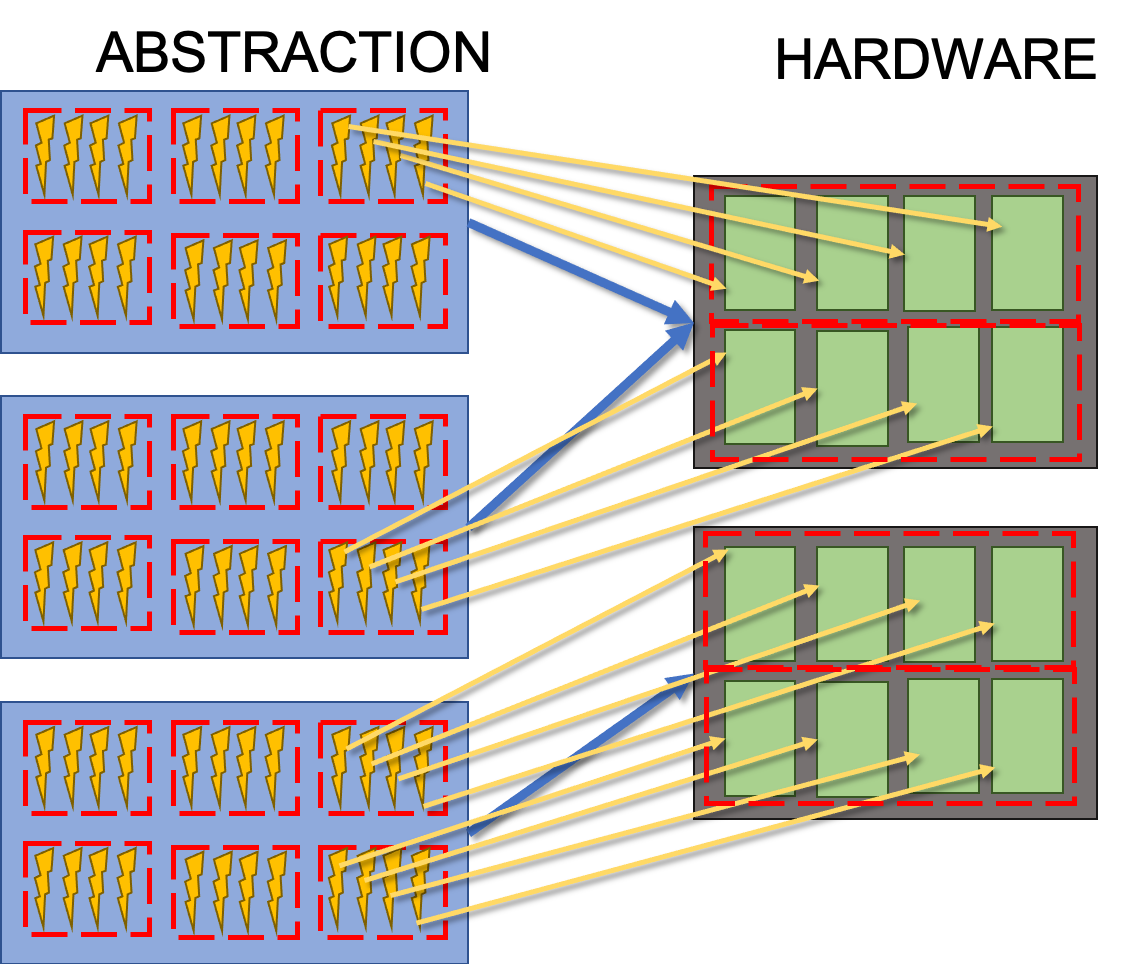
\includegraphics[width=\textwidth]{img/03/gpu-hard-abs.png}
            \end{figure}
        \end{columns}
    \end{frame}

    \begin{frame}{Nested Parallelism on CPU}
        We can also think about nested parallelism on CPU
        \begin{itemize}
            \item Outer: The \texttt{k}, \texttt{i} loops are partitioned between independently-scheduled threads
            \item Inner: The \texttt{j} loop will (hopefully) execute in SIMD
        \end{itemize}
        \begin{block}{}
            \inputminted{c}{src/dgemm-concept.c}
        \end{block}
    \end{frame}

    \section{Exercises}

    \subsection{Running on Midway}

    \begin{frame}{Midway Environment}
        \begin{itemize}
            \item The V100 GPUs are available on "midway".  Older models (K80) are available on "midway2".
            \item Can use either one for today.  Quicker job turnaround on midway2
            \item To compile \textbf{and run}, you need \texttt{module load cuda/8.0}
            \item To run on a GPU node, you need some new SBATCH parameters:
            \begin{block}{}
                \inputminted{bash}{src/midway-gpu.sbatch}
            \end{block}
        \end{itemize}
    \end{frame}

    \subsection{Example 1: Scalar Addition}

    \begin{frame}{Example 1:  Scalar Addition}
        \begin{itemize}
            \item A CUDA program is extended C.
        \end{itemize}
        \begin{block}{}
            \inputminted{cuda}{src/01_scalar_add.cu}
        \end{block}
    \end{frame}

    \begin{frame}{Example 1:  Allocating Device Memory}
        \begin{block}{}
            \inputminted[firstline=7,lastline=9]{cuda}{src/01_scalar_add.cu}
        \end{block}
        \begin{itemize}
            \item \texttt{cudaMalloc} is called from the ``host'' (CPU) to allocate memory on the ``device'' (GPU)
            \item Expects a pointer to \texttt{void *}
            \item The pointer's name is arbitrary (\texttt{dev\_} is just a mnemonic)
            \item After mallocing, the pointer contains an address to \texttt{device memory}, which is a separate virtual address space.
            \item Dereferencing a device pointer in host code has undefined behavior.
        \end{itemize}
    \end{frame}

    \begin{frame}{Example 1:  Allocating Device Memory}
        \begin{block}{}
            \inputminted[firstline=7,lastline=9]{cuda}{src/01_scalar_add.cu}
        \end{block}
        \begin{itemize}
            \item \texttt{cudaMalloc} is called from the ``host'' (CPU) to allocate memory on the ``device'' (GPU)
            \item Expects a pointer to \texttt{void *}
            \item The pointer's name is arbitrary (\texttt{dev\_} is just a mnemonic)
            \item After mallocing, the pointer contains an address to \texttt{device memory}, which is a separate virtual address space.
            \item Dereferencing a device pointer in host code has undefined behavior.
        \end{itemize}
    \end{frame}

    \begin{frame}{Example 1:  The Kernel Function}
        \begin{block}{}
            \inputminted[firstline=1,lastline=3]{cuda}{src/01_scalar_add.cu}
        \end{block}
        \begin{itemize}
            \item A kernel function \texttt{\_\_global} is compiled to run on device and be called by host
            \item \texttt{int *c} is normal pointer datatype, but its value should point an address in device memory.
            \item Dereferencing a host pointer from device code has undefined behavior
            \item The \textbf{same kernel will be run by every active thread}, but not necessarily at the same time
            \item This called \textbf{single-program, multiple-data} (SPMD)
        \end{itemize}
    \end{frame}

    \begin{frame}{Example 1: Launching the Kernel}
        \begin{block}{}
            \inputminted[firstline=11,lastline=11]{cuda}{src/01_scalar_add.cu}
        \end{block}
        \begin{itemize}
            \item This statement calls (launches) a device function (kernel) from the host code
            \item The extra \texttt{<<<dim\_grid, dim\_block>>>} syntax are runtime parameters that specify:
            \begin{itemize}
                %\item The ``grid'' dimensions:  The number of blocks to create
                \item The block dimensions:  The number of threads per block
            \end{itemize}
            \item Here, we run with 1 block containing 1 thread (not actually doing parallel work)
        \end{itemize}
    \end{frame}

    \begin{frame}{Example 1: Copying Data from GPU to Host}
        \begin{block}{}
            \inputminted[firstline=13,lastline=13]{cuda}{src/01_scalar_add.cu}
        \end{block}
        \begin{itemize}
            \item Remember that device data cannot be referenced by host (and vice-versa)
            \item \texttt{cudaMemcpy} will copy data at a device memory address to a host memory address.
            \item There parameters \texttt{cudaMemcpyDeviceToHost} and \texttt{cudaMemcpyHostToDevice} (not shown) control the direction of the memcopy
        \end{itemize}
    \end{frame}

    \begin{frame}{Example 1:  Freeing device memory}
        \begin{block}{}
            \inputminted[firstline=17,lastline=17]{cuda}{src/01_scalar_add.cu}
        \end{block}
        \begin{itemize}
            \item Don't forget to free your device memory!
        \end{itemize}
    \end{frame}

    \begin{frame}{Example 1: Compiling It}
        \begin{block}{}
\texttt{nvcc -O2 01\_scalar\_add.cu -o 01\_scalar\_add}
        \end{block}
        \texttt{nvcc} is the NVIDIA compiler that:
        \begin{itemize}
            \item Uses a normal CPU compiler backend to compile host code
            \item Uses another backend to compile device code to PTX (assembly for NVIDIA GPUs)
        \end{itemize}
        Lots of options to optimize at compile-time ...
    \end{frame}

    \subsection{Block and Thread Indexing}

    \begin{frame}{Hiearchical Block and Thread Indexing}
            \begin{columns}
                \column{0.5\textwidth}
                \begin{itemize}
                    \item Each thread can be uniquely idenftified by a combination of block and thread indices.
                    \item Example: grid dimension = 2 and block dimension = 3
                \end{itemize}
                \column{0.5\textwidth}
                \begin{table}[]
                    \begin{tabular}{|c||c|}
                        \hline
                        blockIdx.x & threadIdx.x \\
                        \hline
                        \hline
                        0          & 0           \\
                        0          & 1           \\
                        0          & 2           \\
                        \hline
                        1          & 0           \\
                        1          & 1           \\
                        1          & 2           \\
                        \hline
                    \end{tabular}
                \end{table}
            \end{columns}
        \end{frame}

    \begin{frame}{Multidimensional Block and Thread Indexing}
        \begin{columns}
            \column{0.4\textwidth}
            \begin{itemize}
                \item Grids and blocks can be structured with up to 3 dimensions each
                \item Example: grid dimension = (2, 2) and block dimension = 3
            \end{itemize}
            \column{0.6\textwidth}
            \begin{table}[]
                \begin{tabular}{|cc||c|}
                    \hline
                    blockIdx.x & blockIdx.y & threadIdx.x \\
                    \hline
                    \hline
                    0          & 0          & 0           \\
                    0          & 0          & 1           \\
                    0          & 0          & 2           \\
                    \hline
                    0          & 1          & 0           \\
                    0          & 1          & 1           \\
                    0          & 1          & 2           \\
                    \hline
                    1          & 0          & 0           \\
                    1          & 0          & 1           \\
                    1          & 0          & 2           \\
                    \hline
                    1          & 1          & 0           \\
                    1          & 1          & 1           \\
                    1          & 1          & 2           \\
                    \hline
                \end{tabular}
            \end{table}
        \end{columns}
    \end{frame}

    \begin{frame}{Limits on Numbers of Threads and Blocks}
        \begin{itemize}
            \item Each GPU generation has limits on the number of threads/block, as well as the sizes of grids and blocks
            \item The limits on a V100 are:
            \begin{itemize}
                \item Max threads/block: 1024
                \item Max block dimensions:  (1024, 1024, 64)
                \item Max grid dimensions: (2147483647, 65535, 65535)
            \end{itemize}
            \item Examples:
            \begin{itemize}
                \item Some allowed block dims:  (1024, 1, 1); (1, 1024, 1); (2, 8, 64)
                \item Disallowed block dims:  (1024, 2, 1) exceeds max threads/block; (4, 2, 128) exceeds block dims
            \end{itemize}
        \end{itemize}
    \end{frame}

    \subsection{Example 2:  A Small Vector Sum}

    \begin{frame}{Example 2:  The Kernel}
        \begin{block}{}
            \inputminted[firstline=6,lastline=11]{cuda}{src/02_vector_add.cu}
        \end{block}
        \begin{itemize}
            \item Recall that every thread runs the same program separately
            \item Threads will have different values for \texttt{blockIdx.x} and \texttt{threadIdx.x}
            \item We uniquely identify each thread by \texttt{i = blockIdx.x * blockDim.x + threadIdx.x} and use \texttt{i} to index the array.
            \item The conditional is necessary to avoid indexing off the edge of the array
        \end{itemize}
        \textbf{Runs in parallel, even though no loops are expressed!}
    \end{frame}

    \begin{frame}{Example 2:  The Host Code}
        \begin{itemize}
            \item Here, we launch the kernel with exactly n threads
            \item Our kernel works with $\ge$ n threads.
            \item Does it work with $<$ n threads?
        \end{itemize}
        \begin{block}{}
            \inputminted[firstline=25,lastline=35]{cuda}{src/02_vector_add.cu}
        \end{block}
    \end{frame}

    \subsection{Example 3: A General Vector Sum}

    \begin{frame}{Example 3:  The Kernel}
        \begin{block}{}
            \inputminted[firstline=6,lastline=12]{cuda}{src/03_large_vector_add.cu}
        \end{block}
        \begin{itemize}
            \item With this for-loop, the threads stride over the array
            \item \textbf{This loop is not done in parallel (not even in SIMD!)}.
            \item The loop is done sequentially by a single thread (remember:  SPMD).
        \end{itemize}
    \end{frame}

    \begin{frame}{Example 4:  Mandelbrot Set}
        \begin{itemize}
            \item In this example, we'll calculate the Mandelbrot Set on GPU
            \item We'll start with our OpenMP implementation from Lecture 2
            \item We'll use a couple new CUDA capabilities:
            \begin{itemize}
                \item \texttt{\_\_device\_\_} attribute:  Declares a function
                      that will be compiled for device and called from device
                \item \texttt{dim3}: A data structure to describe a multi-dimensional layout for grids and blocks (2D layouts also use \texttt{dim3})
            \end{itemize}
        \end{itemize}
    \end{frame}

    \begin{frame}{Example 4: Decomposition Strategy}
        \begin{figure}
            \centering
            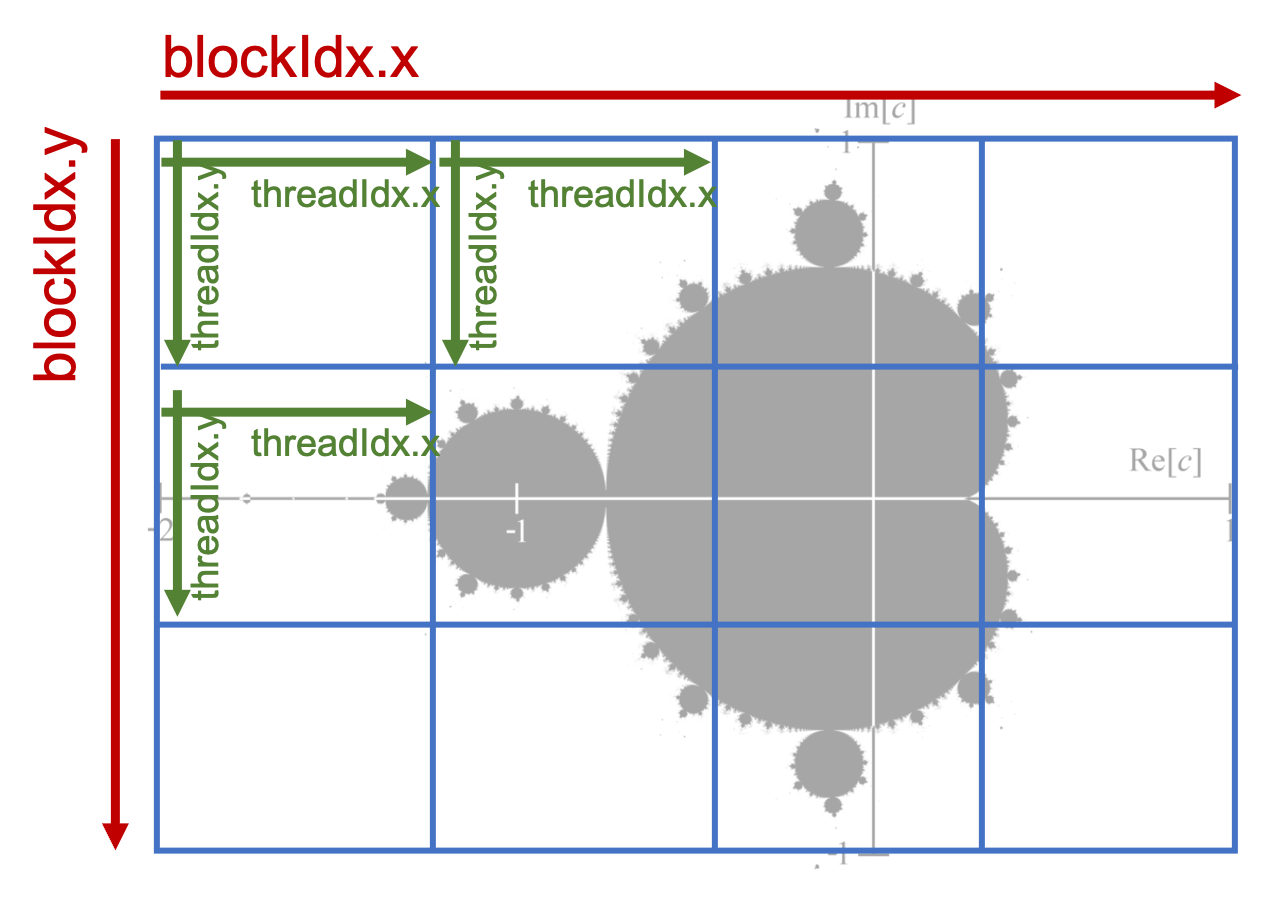
\includegraphics[width=\textwidth]{img/03/mandelbrot.png}
        \end{figure}

    \end{frame}

\end{document}
